\documentclass[oneside]{ausarbeitung}
\bibliography{latexlit}


% ----------------------------------------------------------------------

\begin{document}

%--- Sprachauswahl
% Erlaubte Werte:
%   \selectlanguage{english}
%   \selectlanguage{ngerman}
\selectlanguage{ngerman}

%--- Art der Arbeit
% Erlaubte Werte:
%   \Praxissemesterbericht
%   \Projektbericht
%   \Bachelorarbeit
%   \Seminararbeit
%   \Masterarbeit

\Projektbericht

%--- Studiengang:
% Erlaubte Werte:
%   \Informatik
%   \Elektronik
%   \DataScience
\Informatik

\title{Algorithmisches Handeln von Kryptowährungen}

\author{Sebastian Flum}
\matrikelnr{76855}

%--- Ist der Erstbetreuer (\examinerA) an der Hochschule ein Professor?
% Erlaubte Werte:
%   \examinerIsAProfessortrue   % Ja
%   \examinerIsAProfessorfalse  % Nein
\examinerIsAProfessorfalse

%--- Betreuer
\examinerA{Sebastian Stigler}
%\examinerB{Prof.~Dr.~Ulrich~Klauck}

%--- Einreichungsdatum
\date{28. Februar 2021}

%--- Titelseite Anzeigen
\maketitle
\cleardoublepage

%---
\pagenumbering{roman}
\setcounter{page}{1}

%--- Eidesstattliche Erklärung anzeigen
\makeaffirmation
\cleardoublepage

%---------------------------------------------------
\begin{abstract}
\label{abstract}

Beim algorithmischen Handeln werden Handelsentscheidungen auf der Grundlage zuvor definierter Anweisungen und Regeln getroffen, die in Form eines Computerprogramms umgesetzt wurden. Dabei wird Code geschrieben, der die Trades im Namen des Händlers oder Investors ausführt, wenn bestimmte Bedingungen erfüllt sind. 

Im Rahmen dieser Arbeit wurde versucht, jenes Verfahren auf den Handel von kryptographischen Währungen wie Bitcoin oder Ethereum anzuwenden und den Grundstein eines algorithmisches Handelssystem für diese zu entwerfen. So soll herausgefunden werden, ob der automatisierte Handel von Kryptowährungen, durch ein selbst entwickeltes System, erfolgreich sein kann.

Dabei beschäftigt sich diese Arbeit im grundlegenden mit folgenden Konzepten:

\begin{enumerate}
	\item Algorithmische Handelsstrategien und technische Indikatoren
	\item Implementierung einer Schnittstelle für Handelsplattformen
	\item Backtesting von Handelsstrategien
	\item Erstellung einer Konsolenanwendung
	\item Verknüpfung dieser Elemente innerhalb eines modularen Systems
\end{enumerate}

Umgesetzt wurde dieses Projekt fast ausschließlich unter der objektorientierten Verwendung der Programmiersprache Python, in Verbindung mit einigen wenigen HTML Elementen.

\end{abstract}

%---------------------------------------------------
\cleardoublepage
\tableofcontents

%---
\listoffigures

%---
\listoftables

%---
\listoflistings

%---
\listofabbreviations
\begin{acronym}[API]  % Längstes Kürzel in der nachfolgenden
                       % Liste um die Breite der Spalte für die
                       % Abkürzungen zu bestimmen.

%% Eintrag: \acro{Referenzname}[Kürzel]{Langform}
%% Im Text wird die Abkürzung dann mit \ac{Referenzname} benutzt.
\acro{api}[API]{Application Programming Interface}
\end{acronym}
%---


\cleardoublepage
\pagenumbering{arabic}
\setcounter{page}{1}

%---------------------------------------------------
\chapter{Einleitung}
\label{cha:einleitung}

"Neues Allzeithoch: Bitcoin-Rekordjagd geht ungebremst weiter"\cite{bitcoin_artikel_1}. "Kryptowährung: Bitcoin knackt Marke von 50.000 Dollar"\cite{bitcoin_artikel_2}. Artikel wie diese sind schon lange keine Seltenheit mehr. Kryptowährungen, allen voran der Bitcoin, entwickelten sich in den letzten Jahren zum Sinnbild schnellen Reichtums. Doch das war nicht immer so. Im Jahre 2011, als sich der Bitcoin noch in seinen Kinderschuhen befand, kostete ein Coin gerade einmal 1 Dollar\cite{bitcoin_kurs_2011}. Vielleicht erwischt man sich nun selbst bei dem Gedanken daran, was wohl wäre, wenn man zu dieser Zeit schon das Potential dieser, damals unscheinbaren, Internetwährung erkannt hätte. Einige vorausdenkende Köpfe erkannten dies frühzeitig und wurden dadurch reich. Andere wiederum nutzten die neu entdeckte Kryptowährung dazu, online für ihre Pizza zu bezahlen. Verrückt, wenn man sich vor Augen führt, dass man mit der selben Menge Bitcoins heute zehntausende Pizzen bezahlen könnte. Vielleicht lässt dieser Gedanke die Herzen einiger Pizzaliebhaber höher schlagen, vorrangig stellt sich jedoch die Frage, ob man mit dem Besitz und Handel von Kryptowährungen heutzutage noch Erfolg haben kann. Und wenn ja - kann das auch ein Computerprogramm?

\section{Motivation}
\label{sec:motivation}

Natürlich stellt die Aussicht auf realisierbaren Gewinn, erzeugt durch ein selbst entwickeltes Handelssystem, ein großer Motivationsfaktor dar - doch es ist mehr als das. Kryptowährungen liegen einem faszinierendem Stück Technologie zugrunde. Der sogenannten \textbf{Blockchain} (dazu später mehr). Dennoch können die digitalen Währungen wie jede herkömmliche Währung getauscht und gehandelt werden, befinden sich gleichzeitig aber außerhalb der Kontrolle finanzieller Institutionen. Somit verbinden Kryptowährungen die Welt des Finanzhandels mit der Welt der Informatik. Für jemanden, den der herkömmliche Handel mit Wertpapieren oder Ähnlichem nur wenig anspricht, bieten Kryptowährungen die Möglichkeit eines interessanten Einblicks in beide Welten. 

Abgesehen davon finde ich großen Gefallen daran, Lösungen für gegebene Problemstellungen zu entwerfen und in Programmcode umzusetzen. Es macht mir Spaß, neue Technologien kennenzulernen und deren Konzepte praktisch einzusetzen. Der Entwurf eines algorithmischen Handelssystems bietet dafür die perfekte Grundlage, da es beliebig erweitert werden kann und viele Schlüsselkonzepte vereint. So stellt das Projekt eine interessante Möglichkeit für mich dar, Dinge wie objektorientierte Programmierung, Entwurf von Softwarearchitekturen und Datenbanken, Web-Entwicklung und vielem mehr, innerhalb eines zusammenhängenden Projektes, kennenzulernen und anzuwenden.

\section{Problemstellung und -abgrenzung}
\label{sec:problemstellung}

Als Ganzes betrachtet ist die Problemstellung, ein algorithmisches Handelssystem zu entwerfen, relativ unüberschaubar. Zur Bewältigung muss es daher in mehrere Teilprobleme heruntergebrochen werden. Daraus ergeben sich folgende, im nachfolgenden grob beschriebene, Problemstellungen:

\textbf{1. Algorithmische Handelsstrategien und technische Indikatoren} \\
Ohne eine geeignete Trading-Strategie, die entscheidet, wann Einkäufe und Verkäufe zu tätigen sind, kann wohl kein System Erfolg haben. Diesen Trading-Strategien liegen technische Indikatoren zu Grunde. Ein technischer Indikator dient dabei zur alternativen Darstellung der Kursverläufe liefert der Strategie wertvolle Analyseinformationen. Der Fokus soll dabei jedoch weniger auf der Findung und Konzeption neuer Strategien und Indikatoren liegen, sondern darauf, wie diese möglichst einfach und modular in das System eingebunden werden können.

\textbf{2. Implementierung einer Schnittstelle für Handelsplattformen} \\
Der Handel von Kryptowährungen mittels eines algorithmischen Systems erfordert, genauso wie beim Handeln von Hand, eine Plattform, auf der die Ein- und Verkäufe getätigt werden. Im Vergleich zum Handeln von Hand, benötigt das Trading-System jedoch eine Schnittstelle \ac{api}, an die es anknüpfen kann, um mögliche Aktionen der Plattform tätigen zu können. Einige Plattformen bieten solche APIs zum Teil kostenlos an. Die Problemstellung ergibt sich daraus, die von den Plattformen bereitgestellten APIs zu nutzen und eigene, möglichst modulare, Schnittstellen zur Verwendung dieser zu entwerfen.

\textbf{3. Backtesting von Handelsstrategien} \\
Backtesting bzw. Rückvergleich bezeichnet den Prozess, eine Strategie zu evaluieren, indem die Strategie auf historische Daten angewandt wird. Findet man beispielsweise eine neue, vielversprechende Trading-Strategie und möchte diese nun nach der Umsetzung in Code testen, ist es sehr riskant, die Strategie im Echtzeitbetrieb laufen zu lassen. Sollte die Strategie nämlich doch nicht so vielversprechend sein, läuft man Gefahr, große Verluste durch schlecht platzierte Ein- und Verkäufe hinnehmen zu müssen. Der Backtest wirkt diesem Risiko entgegen und stellt somit eine der wichtigsten Komponenten des Systems dar. 

\textbf{4. Erstellung einer Konsolenanwendung} \\
Alle Features des zu entwickelnden Systems, sollen dem Nutzer als Teil einer Konsolenanwendung zur Verfügung stehen. Mit dieser soll es beispielsweise möglich sein, Backtests sowie neue "Händler-Instanzen" aka Trading-Bots zu erstellen, welche verschiedenen Parametern wie Auswahl der Kryptowährung, Strategie, Kapital, usw. zu Grunde liegen.

\textbf{5. Verknüpfung der Komponenten innerhalb eines modularen Systems} \\
Im laufe der Arbeit werden Lösungskonzepte für die, hier aufgeführten, Problemstellungen entworfen und implementiert. Wichtig ist es dabei, die Komponenten mit Hinblick auf das Gesamtsystem und dessen Erweiterbarkeit/Modularität zu entwerfen, sowie ein sauberes und klar definiertes Zusammenspiel zu ermöglichen. 

\section{Ziel der Arbeit}
\label{sec:ziel}

Wie sich aus den vorherigen Abschnitten bereits erkennen lässt, stellt das Ziel dieser Arbeit den Entwurf und die Implementierung eines algorithmischen Handelssystems für Kryptowährungen dar. Dabei soll es dem System möglich sein, Marktdaten über Kryptowährungen zu sammeln und automatisiert auszuwerten. Des weiteren soll das System über eine Teststrategie sowie den dazugehörigen technischen Indikatoren enthalten, welche durch einen, ebenfalls im System implementierten, Backtest ausgewertet werden kann. Dabei soll es dem System möglich sein, ausgewählte Markdaten und Backtest-Ergebnisse zu visualisieren und anschaulich darzustellen. Unter anderem soll das System einen Prototyp eines Trading-Bots enthalten, welcher mit zukünftigen Erweiterungen in der Lage sein soll, echte Handelsaktionen durchzuführen. All diese Funktionen sollen dem Nutzer durch eine Konsolenanwendung bereitgestellt werden.

\section{Vorgehen}
\label{sec:vorgehen}

Nachdem mit Problemstellung und Ziel gewissermaßen Anfangs- und Endpunkt 
des Praktikums beschrieben sind, wird hier der zur Erreichung des Ziels 
eingeschlagene Weg vorgestellt. Dazu werden typischerweise die folgenden 
Kapitel und ihr Beitrag zur Erreichung des Ziels der Arbeit kurz 
beschrieben. Die folgenden Kapitel sind ein – möglicher – Aufbau, 
Abweichungen können durchaus notwendig sein. Zur Darstellung des 
Vorgehens ist eine grafische Darstellung sinnvoll, bei der die einzelnen 
Lösungsschritte und ihr Zusammenhang dargestellt werden. Ein Beispiel 
hierfür findet sich in Abbildung \ref{fig:1}.

\begin{figure}[htbp]
  \centering
  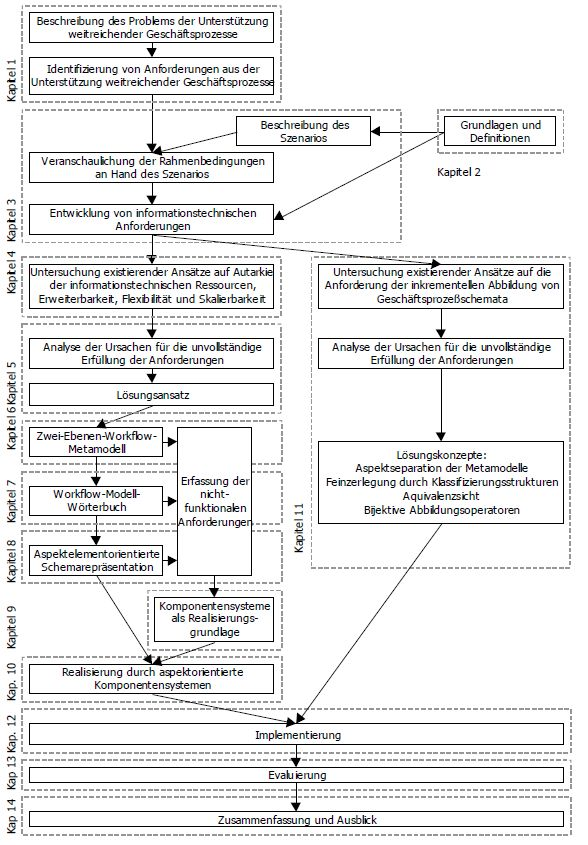
\includegraphics[height=0.9\textheight]{img/ausarbeitung.jpg}
  \caption{vorgehen nach \autocite{Schmidt:Geschaeftsprozesse}}
  \label{fig:1}
\end{figure}

%---------------------------------------------------
\chapter{Grundlagen}
\label{cha:grundlagen}

In diesem Kapitel das für das Praktikum relevante Grundlagenwissen 
dargestellt. Der Praktikant soll hierzu das ihm durch Vorlesungen 
bekannte, bzw. durch Recherchen vertiefte theoretische Wissen 
darstellen, das für die Lösung der im Praktikum gestellten Probleme 
notwendig ist.

Dabei ist darauf zu achten, nur solche Inhalte in das Grundlagenkapitel 
aufzunehmen, die später auch verwendet werden (Problembezogenheit). 
Ebenso ist auf eine ausreichend tiefe und vollständige Darstellung der 
Grundlagen zu achten.

Für die Erstellung des Literaturverzeichnisses 
wird das Werkzeug JabRef\autocite{JabRef:JabRef} verwendet. 

Sie können aber auch das Werkzeug Citavi\autocite{SAS:Citavi} benutzen
und dort nach \textsc{Bib}\TeX{} exportieren.

%----
\section{Trading}
\label{sec:trading}

Das Wort "Trading", zu Deutsch: Handel, stammt aus dem Englischen und beschreibt den Kauf und Verkauf von Finanzprodukten an einer Börse. Menschen, die dieser Beschäftigung nachgehen, werden daher auch als Trader bezeichnet. Ein durchgeführter Handel heißt dementsprechend also Trade. (vgl. \cite{trading_1})

Trading bedeutet, die Schwankungen der Finanzmärkte mithilfe von Trades für die eigenen Zwecke zu nutzen. Das heißt kaufen, verkaufen und dabei Gewinne einstreichen - oder den Verlust verkraften. Durch das Internet und benutzerfreundliche Trading-Anbieter ist es auch für Hobby-Anleger möglich, Finanzinstrumente wie Wertpapiere, Währungen, Rohstoff-Zertifikate oder Ähnlichem zu handeln. Beim Trading handelt es sich grundsätzlich um Spekulation. Wo ein Trader sein Geld investiert, ist meist von untergeordneter Wichtigkeit. Beispielsweise geht es nicht darum, Anteile eines Unternehmens zu kaufen, um langfristig an dessen Entwicklung teilzuhaben. Das Ziel eines Traders ist es, durch einen Kursanstieg im Zeitraum des Besitzes eins Finanzinstruments Gewinn zu erzielen. Das bedeutet, ein Trader kauft beispielsweise eine Aktie, hofft auf einen Kursanstieg und verkauft sie dann wieder. Die anschließende Wertdifferenz abzüglich der Transaktionskosten stellt den Gewinn des Traders dar. (vgl. \cite{trading_2})

\subsection{Algorithmischer Handel}
\label{sub:algorithmischer_handel}

Algorithmischer beschreibt den automatischen Handel von Finanzinstrumenten durch Computerprogramme. 

\subsection{Finanzdiagramme}
\label{sub:finanzdiagramme}

\subsection{Technische Indikatoren}
\label{sub:technische_Indikatoren}

\subsection{Trading-Strategien}
\label{sub:trading_strategien}

%----

\section{Kryptowährungen}
\label{sec:kryptowährungen}

\subsection{Funktionsweise}
\label{sub:blockchain}

\subsection{Handel von Kryptowährungen}
\label{sub:handel_von_kryptowährungen}

%----

\section{Python}
\label{sec:python}

\subsection{Vorteile}
\label{sub:vorteile}

\subsection{Einsatzgebiete}
\label{sub:einsatzgebiete}

%----

\section{HTML}
\label{sec:html}

%----

\section{Versionierung}
\label{sec:versionierung}

\subsection{Git}
\label{sub:git}

\subsection{Gitflow}
\label{sub:gitflow}

%---------------------------------------------------
\chapter{Problemanalyse}
\label{cha:problemanalyse}

Die Analyse des zu lösenden Problems ist Grundlage für jedes 
ingenieurmäßige Vorgehen. Daher soll in diesem Kapitel das zu lösenden 
Problem auf Basis des im Grundlagenkapitel aufbereiteten Wissens 
analysiert werden. Hierzu ist insbesondere notwendig zu klären, wie sich 
das Gesamtproblem in Teilprobleme zerlegen lässt und welche 
Abhängigkeiten zwischen diesen bestehen.

Bei Software-Projekten befindet sich an dieser Stelle typischerweise die 
Anforderungsanalyse des \ac{rup}.

%---
\chapter{Lösungskonzept}
\label{cha:loesungskonzept}

Auf der Basis der im vorangegangenen Kapitel erstellten Problemanalyse 
und der im Grundlagenkapitel aufgearbeiteten theoretischen Kenntnisse 
wird ein Lösungskonzept erarbeitet.

Bei Software-Projekten entspricht dieses Kapitel typischerweise der 
Analyse \& Design-Phase des \ac{rup}. Typische Ergebnisse dieser Phase sind 
Klassendiagramme etc.

%---
\chapter{Implementierung}
\label{cha:implementierung}

In diesem Kapitel wird die konkrete Implementierung des im Kapitel
\ref{cha:loesungskonzept} entwickelten Lösungskonzepts beschrieben.
Hierbei wird auf die konkret verwendeten Entwicklungswerkzeuge etc. 
Bezug genommen.

Bei Software-Projekten besteht dieses Kapitel typischerweise aus den 
Phasen Implementierung \& Test im \ac{rup}.

Zum Beispiel kann man hier auch ein kleines Listing einfügen.

\begin{lstlisting}[language=c,%
                   caption={Überschrift des Quelltexts}]
#include<stdio.h>

int main() {
    // Kommentar
    int answer = 20 << 1;
    answer += 2;
    printf("Hallöchen Welt!\n");
    printf("Die Antwort ist: %d\n", answer);
    return 0;
}
\end{lstlisting}

Manchmal hilft auch eine kleine Tabelle:

\begin{table}[htbp]
\centering
\begin{tabular}{|l|r|}
\hline
\textbf{Messwert a} & \textbf{Messwert b} \\ \hline
9 & 5 \\ \hline
1 & 4 \\ \hline
1 & 3 \\ \hline
\end{tabular}
\caption{Überschrift der Tabelle}
\label{tab:my-table}
\end{table}

Details siehe Tabelle~\ref{tab:my-table}.
%---
\chapter{Inbetriebnahme}
\label{cha:inbetriebnahme}

Aufgabe des Kapitels Inbetriebnahme ist es, die Überführung der in 
Kapitel \ref{cha:implementierung} entwickelte Lösung in das betriebliche 
Umfeld aufzuzeigen. Dabei wird beispielsweise die Inbetriebnahme eines 
Programms beschrieben oder die Integration eines erstellten 
Programmodules dargestellt.

Bei der Software-Erstellung entspricht dieses Kapitel der 
Auslieferungsphase (Deployment) im \ac{rup}.

%---
\chapter{Evaluierung}

Aufgabe des Kapitels Evaluierung ist es, in wie weit die Ziele der 
Arbeit erreicht wurden. Es sollen also die erreichten Arbeitsergebnisse 
mit den Zielen verglichen werden. Ergebnis der Evaluierung kann auch 
sein, das bestimmte Ziele nicht erreicht werden konnten, wobei die 
Ursachen hierfür auch außerhalb des Verantwortungsbereichs des 
Praktikanten liegen können.

%---
\chapter{Zusammenfassung und Ausblick}
\label{cha:zusammenfassung}

\section{Erreichte Ergebnisse}
\label{sec:ergebnisse}

Die Zusammenfassung dient dazu, die wesentlichen Ergebnisse des 
Praktikums und vor allem die entwickelte Problemlösung und den 
erreichten Fortschritt darzustellen. (Sie haben Ihr Ziel erreicht und 
dies nachgewiesen).

\section{Ausblick}
\label{sec:ausblick}

Im Ausblick werden Ideen für die Weiterentwicklung der erstellten Lösung 
aufgezeigt. Der Ausblick sollte daher zeigen, dass die Ergebnisse der 
Arbeit nicht nur für die in der Arbeit identifizierten Problemstellungen 
verwendbar sind, sondern darüber hinaus erweitert sowie auf andere 
Probleme übertragen werden können.

\subsection{Erweiterbarkeit der Ergebnisse}
\label{sub:erweiterbarkeit}

Hier kann man was über die Erweiterbarkeit der Ergebnisse sagen.

\subsection{Übertragbarkeit der Ergebnisse}
\label{sub:uebertragbarkeit}

Und hier etwas über deren Übertragbarkeit.

%-----------------------------------------------------------------------
\appendix

%---
\printbibliography[heading=bibintoc]

%---
\chapter{Anhang A}

%---
\chapter{Anhang B}


\end{document}